% Prof. Dr. Ausberto S. Castro Vera
% UENF - CCT - LCMAT - Curso de Ci\^{e}ncia da Computa\c{c}\~{a}o
% Campos, RJ,  2022
% Disciplina: An\'{a}lise e Projeto de Sistemas
% Aluno: 

\chapterimage{analise.png} % Table of contents heading image
\chapter{Etapa de An\'{a}lise}

Neste capítulo é apresentada a análise do sistema, que é composta pela coleta e apresentação de
requisitos, seleção de stakeholders, entrevista, casos de uso, diagramas de fluxo de dados e diagrama
de entidades e relacionamentos.


\section{Requisitos do Sistema}

Nesta seção serão listados os requisitos do sistema além de algumas de suas definições e especificações.

\subsection{Requisitos}
\begin{enumerate}
  \item Computadores para todos o setores
  \item Servidores
  \item Rede interna para todos os setores
  \item Gerenciamento de controle de estoque
  \item impressão de relatórios
  \item Acesso a internet
  \item Acesso ao sistema
  \item Cadastro de clientes
  \item Controle de vendas
  \item Catálogos de produtos
  \item Gerenciamento de finanças Setor administrativo
  \item Gerenciamento de fornecedores
  \item Sistema de segurança
  \item Anti-vírus
  \item Suporte ao pacote office
  \item Sistemas operacionais atualizados
  \item Criação do site
  \item Vendas e entrega online
  \item Disponibilidade de produtos
  \item Cadastro de clientes online
  \item Gerenciamento de entrega
  \item Programa de gerenciamento de dados
  \item Gerenciamento de varias formas de pagamento
  \item Serviço de e-mail
  \item Confidencialidade de dados em geral
  \item Analista de sistema
  \item Programadores
  \item Engenheiro de software
  \item Funcionários
  \item Equipe treinada para o uso do sistema
  \item Manual do sistema
  \item Treinamento de funcionários
  \item Contabilizar horas de trabalho dos funcioários
  \item Atendimento a padrões
  \item Backup diários na nuvem
  \item Interface didática
  \item Interface acessivel
  \item Sistema rápido e dinâmico
  \item Comunicação entre setores
  \item Comunicção entres todas as unidades
  \item Sincronização de dados entre unidades
  \item Criação do aplicativo
  \item Disponibilização de promoções no aplicativo
  \item Cadrasto de passagens no aplicativo
  \item Controle de passagens
  \item Controle de aeronaves
  \item Vendas e entregas pelo aplicativo
  \item Manutenção rotineira
  \item Resultados de orçamentos
  \item Tolerância a falhas
  \item Gerenciamento de localizção de unidade mais proxima
        
\end{enumerate}



\subsection{Definições de Requisitos}
\begin{enumerate}

  \item[1.] \textbf{Computadores em todos os aeroportos} - Deverá ser feita a instalação e manutenção de
        computadores em todas aos aeroportos, com acesso a internet e conectados em rede\\      
  \item[3.] \textbf{Controle de vendas} - vendas de passagens devem ser registradas no sistema, alterando
        o estoque e sendo associadas a contas de usuários cadastrados\\
  \item[8.] \textbf{Segurança} - o sistema deve ser  capaz de prevenir erros e perdas de dados\\
  \item[10.] \textbf{Gerenciamento de viagens} - a logística das viagens devem partir dos dados de
        proximidade do proximo aeroporto e pelo destino dos passageiros passageiros\\
  \item[24.] \textbf{Construção do sistema de vendas} - Sistema interno de vendas \\
  \item[26.] \textbf{Contrução do web-site de vendas} - Sistema onde os clientes fazem a compra \\
  \item[35.] \textbf{Geração de relatórios automatizados} - o sistema deve gerar relatórios automatizados
        com dados sobre passagens, vendas, viagens, passageiros, faturamento, gastos.\\
  \item[39.] \textbf{Gerenciamento de aviões} - Sistema irá gerenciar todos os detalhes sobre as aeronaves\\
  \item[40.] \textbf{Sincronização de dados entre filiais} - o sistema deve estar sempre sincronizado de
        forma a prevenir erros e gastos desnecessários entre as viagens.
  \item[41] \textbf{Analise de passageiros} - Sistema irá fazer uma analise grafica para verificar o tipo
        de passageiro que voa na sua empresa, gerando um relatorio automatizados\\
  \item[48] \textbf{Analise de viagens} - Sistema irá fazer uma analise grafica para verificar o tipo
        alguns pontos patronizados dentro das viagens para futuras modificações.\\
  \item[79] \textbf{Construção do sistema de aeronaves} - Sistema interno de verificaçãos
        das informações das aeronaves \\
  \item[80] \textbf{Sistema de gerenciamendo de banco de dados} - Para armazenamentos dos dados utilizando as tecnologias mais adequadas
\end{enumerate}


\subsection{Especificações de requisitos}
\begin{enumerate}
  \item[1.] \textbf{Controle de vendas}
        \subitem{
          \begin{enumerate}
            \item[1.1] Passagem cadastrada no sistema
            \item[1.2] Cliente cadastrado no sistema de compra
            \item[1.3] Cadastro de venda é realizado em função ao cliente
            \item[1.5] Processamento desse cadastro dentro do banco de dados
            \item[1.6] Conclusão da venda
            \item[1.8] Atualização do numero de milhas do passageiro
            \item[1.7] Com as informações será feito a análise gráfica \\
          \end{enumerate}
        }
        
  \item[2.] \textbf{Integração entre aeroportos}
        \subitem{
          \begin{enumerate}
            \item[2.1] Lista de todas as filiais existentes
            \item[2.2] Inserção de todos as filiais dentro do sistema
            \item[2.3] Cadastro dos dados de cada aeroporto no sistema geral
            \item[2.4] Utilização de um banco de dados unico
            \item[2.5] Geração de relatorio automatizado se todas as agencias
            \item[2.6] Alerta de disponibilidade de estoque em outras unidades \\
          \end{enumerate}
        }
  \item[3.] \textbf{Banco de dados}
        \subitem{
          \begin{enumerate}
            \item[3.1] Criação do diagrama do banco de dados para cada entidade
            \item[3.2] Criar as relações e o numero de relacionamentos
            \item[3.3] Adicionar atributos para cada entidade
            \item[3.4] Desenvolvimento do banco para utilização do sistema
            \item[3.5] Desenvolvimento do Backup do bando de dados
            \item[3.6] Integração com o Back-end do sistema \\
          \end{enumerate}
        }
  \item[4.] \textbf{Sistema de análise de dados}
        \subitem{
          \begin{enumerate}
            \item[4.1] Consultas desejadas a se fazer para analise
            \item[4.2] Busca e tratamento das informações
            \item[4.3] Desenvolvimento dos graficos para a analise
            \item[4.4] Desenvolvimento dos relatórios
            \item[4.5] Utilização de um Gateway para deixar os relatorios automatizados
            \item[4.6] Implementação para o gerente ou gestores receberem os relatorios mensalmente\\
          \end{enumerate}
        }
  \item[5.] \textbf{Geração de relatórios automatizados}
        \subitem{
          \begin{enumerate}
            \item[4.1] Separação dos tipos de relatorios desejados
            \item[4.2] Sistema de dados para auxiliar os relatorios
            \item[4.3] Cada analise terá informações complementares para o entendimento
            \item[4.4] Alerta sobre informações importantes dentro do relatorio
            \item[4.5] Envio do relatorio mensalmente para os gestores\\
          \end{enumerate}
        }
\end{enumerate}




\section{Stakeholders e Pontos de Vista}
Nesta seção estão presentes os diagramas de requisitos 
buscam representar os requisitos anteriormente apresentados de forma gráfica.

\subsection{Stakeholders}


\begin{itemize}
  \item Passageiros
  \item Gerente de cada companhia
  \item Funcionarios
  \item Pilotos
  \item Gestão Financeira
  \item Departamento de controle de aeronaves
  \item Departamento de vendas
  \item Gerente de analise gráfica \\
\end{itemize}





\section{Entrevista}
A entrevista é uma ferramenta muito importante na criação de um sistema, pois é uma forma de
contato com stakeholders muito real, e que retorna requisitos imediatos observados na condução da
entrevista.

Foram selecionadas oito perguntas com o intuito de descobrir contras do sistema antigo, para a
melhoria dos mesmo. E prós para a manutenção e aprimoramento no novo sistema. Além de
perguntas que buscam entender o que é importante para os funcionários que utilizam o sistema,
e quais as principais necessidades dos mesmos. A entrevista foi feita com um funcionário que
trabalha no balcão de uma das farmácias, e que está constantemente lidando com o sistema de
gerenciamento de estoque e recebimento de pedidos.


\section{ Casos de Uso}



\section{Modelagem do Sistema}


\subsection{Modelagem de Processos}


\subsection{Modelagem de Dados}

\section{Diagrama de entidades e relacionamentos}
O diagramas a seguir representam a modelagem de relacionamento entre as entidades do sistema.


  \caption{Diagrama de entidade}
  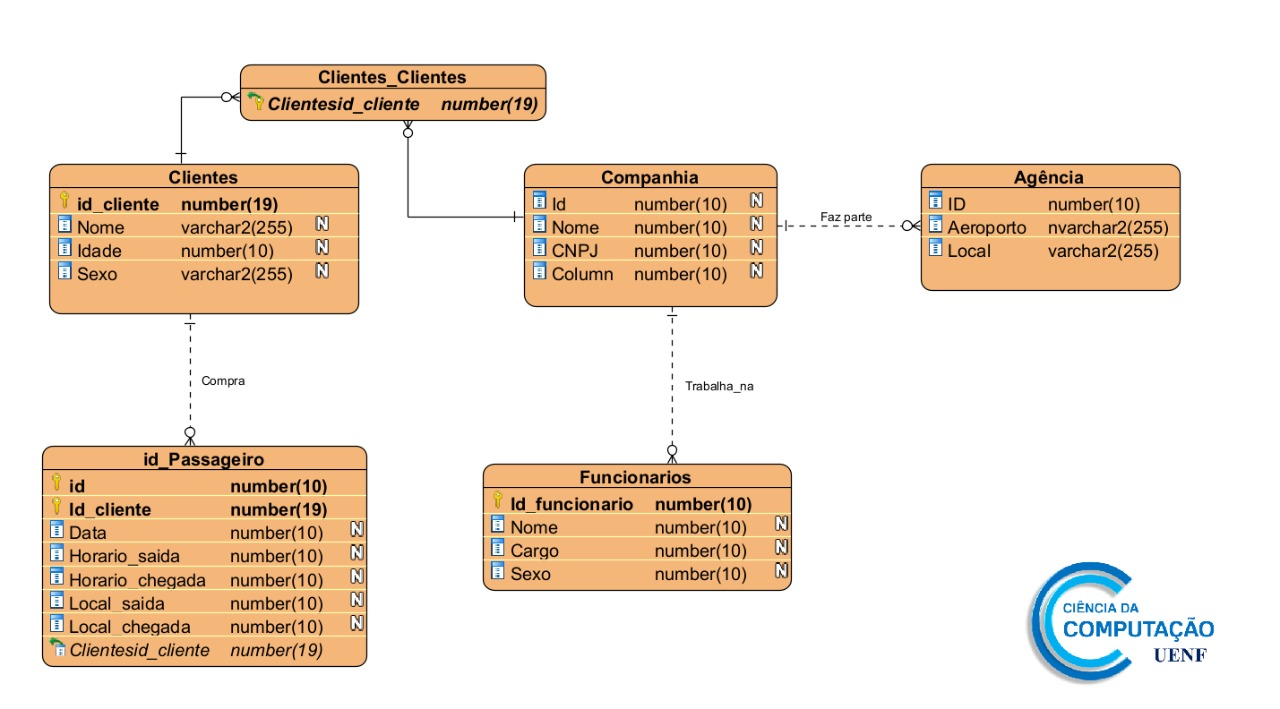
\includegraphics[width=16cm]{Diagrama.jpeg}
